\documentclass[12pt]{memoir}
\usepackage{amsmath}
\usepackage{authblk}
\usepackage{xcolor}
\usepackage{mdframed}
\usepackage{tikz}
\usepackage{fancyhdr}
\usepackage{calc}
\usepackage{marginnote}
\usepackage{graphicx}
\usepackage{hyperref}

% Set the left and right margin for the header
\setlength{\headwidth}{2cm+\evensidemargin}
\pagestyle{fancy}
\fancyhf{} % Empty Headers
\fancyhead[LE]{\thepage} % Page number on left for even pages
\fancyhead[RO]{\thepage} % Page number on right for odd pages
\fancyhead[RE]{Communicating without errors} % Header on even pages
\fancyhead[LO]{Communicating without errors} % Header on odd pages

\renewcommand{\headrulewidth}{0.4pt} % Thickness of the header rule


% Redefine \theequation to exclude chapter number
\renewcommand{\theequation}{\arabic{equation}}


% Define a new environment for quotes
\newmdenv[
  backgroundcolor=white,
  linewidth=0pt,
  innerleftmargin=8pt,
  innertopmargin=10pt,
  innerrightmargin=0pt,
  innerbottommargin=10pt,
  leftmargin=-10pt,
  skipabove=\topsep,
  skipbelow=\topsep,
  frametitle={\tikz[overlay,remember picture] \node[anchor=north east,rectangle,fill=gray!60,inner sep=4pt] at (frame.north east) {};}
]{quotebox}

\setlrmarginsandblock{0.5cm}{8cm}{*}
\setulmarginsandblock{0}{0cm}{*}
\checkandfixthelayout

% Define margins for the second page onward
\newcommand{\setsecondpagemargins}{
    \clearpage
    \setulmarginsandblock{2cm}{0.5cm}{*}
    \checkandfixthelayout
}


\newenvironment{myquote}
{\begin{quotebox}\begin{quote}}
{\end{quote}\end{quotebox}}

\begin{document}
\setcounter{chapter}{32}

% Adjust space before and after chapter title
\setlength{\beforechapskip}{5pt} % Adjust as needed
\setlength{\afterchapskip}{55pt} % Adjust as needed

\chapter{Communicating without errors}

% Add an image in the right margin
\marginnote{\hspace*{10pt}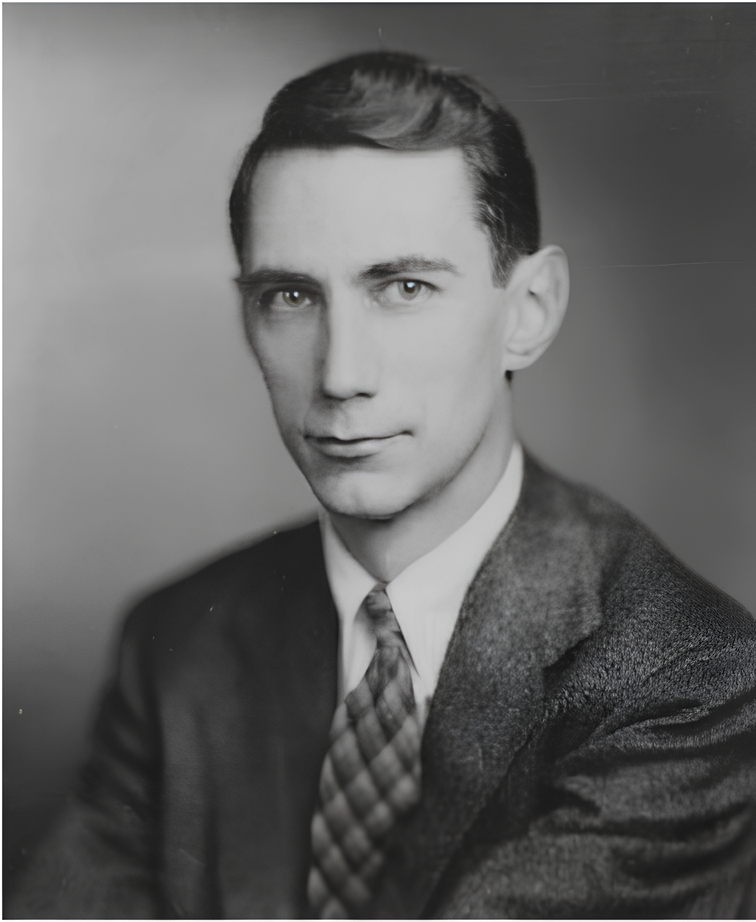
\includegraphics[width=\marginparwidth-30pt]{images/shannon.jpg}\\\hspace*{10pt}Claude Shannon}[0pt]
\marginnote{\hspace*{0pt}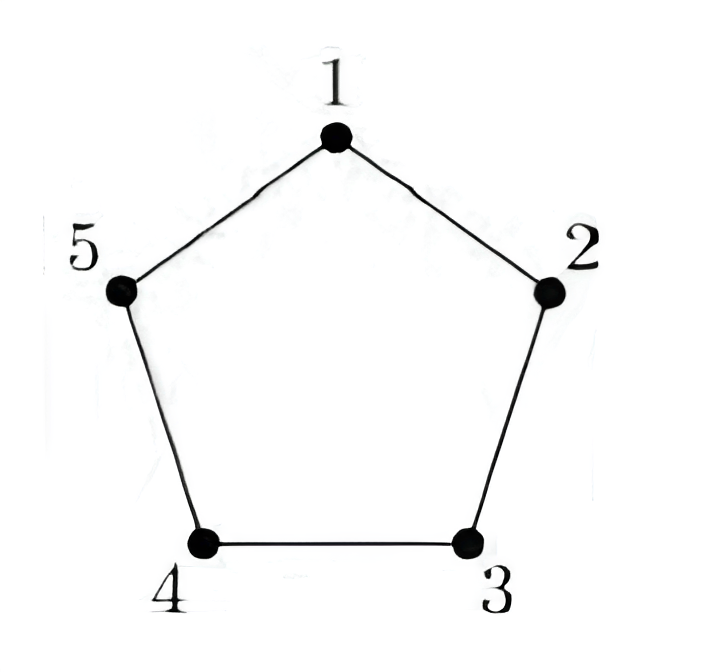
\includegraphics[width=125pt]{images/C5.png}}[267pt]

In 1956 Claude Shannon, the founder of information theory, posed the following very interesting question:

\begin{myquote}
\textit{Suppose we want to transmit messages across a channel (where 
some symbols may be distorted) to a receiver: What is the maximum
rate of transmission such that the receiver may recover the original
message without errors?}
\end{myquote}

\noindent Let us see what Shannon meant by ``channel" and ``rate of transmission." 
We are given a set V of symbols, and a message is just a string of symbols 
from V. We model the channel as a graph $G = (V,E)$  where $V$ is the set 
of symbols, and $E$ the set of edges between unreliable pairs of symbols, 
that is, symbols which may be confused during transmission. For example, 
communicating over a phone in everyday language, we connnect the symbols
$B$ and $P$ by an edge since the receiver may not be able to distinguish 
them. Let us call $G$ the \textit{confusion graph}.
The 5-cycle $C_5$ will play a prominent role in our discussion. In this example,
$1$ and $2$ may be confused, but not $1$ and $3$, etc. Ideally we would like 
to use all $5$ symbols for transmission, but since we want to communicate error-free we can 
if we only send single symbols use only one letter from each pair that might
be confused. Thus for the 5-cycle we can use only two different letters
(any two that are not connected by an edge). In the language of information theory,
this means that for the 5-cycle we achieve an information rate of
$\log_2 2 = 1$ (instead of the maximal $\log_2 5 \approx 2.32$). It is clear that in this model,
for an arbitrary graph $G = (V, E)$, the best we can do is to transmit symbols from
a largest independent set. Thus the information rate, when sending single symbols,
is $log_2 \alpha(G)$, where $\alpha(G)$ is the \textit{independence number} of $G$.

\noindent Let us see whether we can increase the information rate by using larger 
strings in place of single symbols. Suppose we want to transmit strings of 
length 2. The strings ulu2 and vlv, can only be confused if one of the 
following three cases holds: 

\begin{itemize}
  \item $u_1 = v_1$ and $u_2$ can be confused with $v_2$,
  \item $u_2 = v_2$ and $u_1$ can be confused with $v_1$, or
  \item $u_1 \neq v_1$ can be confused and $u_2 \neq v_2$ can be confused. 
\end{itemize}

\noindent In graph-theoretic terms this amounts to considering the product $G_1 \times G_2$ 
of two graphs $G_1 = (V_1, E_1)$  and $G_2 = (V_1, E_1)$. $G_1 x G_2$ has the vertex

\setsecondpagemargins

\noindent set $V_1 \times V_2 = \{(u_1,u_2) :\ u_1 \in V_1,u_2 \in V_2\}$, with $(u_1,u_2) \neq (v_1,v_2)$ 
connected by an edge if and only if $u_i = v_i$ or $u_iv_i \in E$ for $i = 1,2$. The 
confusion graph for strings of length $2$ is thus $G^2 - G \times G$, the product of 
the confusion graph $G$ for single symbols with itself. The information rate 
of strings of length $2$ \textit{per symbol} is then given by

\begin{equation*}
  \frac{\log_2 \alpha(G^2)}{2} = \log_2\sqrt{\alpha(G^2)}.
\end{equation*}

\noindent Now, of course, we may use strings of any length $n$. The $n$-th confusion 
graph $G^n = G \times G \times\dotsb\times G$ has vertex set $V^n = \{(u_1,\dotsb,u_n) : u_i \in V\}$ 
with $(u_1,\dotsb,u_n) \neq (v_1,\dotsb,v_n)$ being connected by an edge if $u_i = v_i$ or 
$u_iv_i\ \in\ E$ for all $i$. The rate of information per symbol determined by 
strings of length $n$ is

\begin{equation*}
  \frac{\log_2 \alpha(G^n)}{n} = \log_2\sqrt[n]{\alpha(G^n)}.
\end{equation*}

\noindent What can we say about $\alpha(G^n)$? Here is a first observation. Let $U \subseteq V$ 
be a largest independent set in $G$, $|U| = \alpha$. The an vertices in $G^n$ of the 
form $(u_1, \dotsb , u_n)$, $u_i \in U$ for all $i$, clearly form an independent set in $G^n$.
Hence 

\begin{equation*}
  \alpha(G^n) \geq \alpha(G)^n
\end{equation*}

\noindent and therefore

\begin{equation*}
  \sqrt[n]{\alpha(G^n)} \geq \alpha(G),
\end{equation*}

\noindent meaning that we never decrease the information rate by using longer strings 
instead of single symbols. This, by the way, is a basic idea of coding theory: 
By encoding symbols into longer strings we can make error-free communi- 
cation more efficient.
Disregarding the logarithm we thus arrive at Shannon's fundamental 
definition: The \textit{zero-error capacity} of a graph $G$ is given by 


\begin{equation*}
  \Theta(G) := \sup_{n\geq1}\sqrt[n]{\alpha(G^n)},
\end{equation*}

\marginnote{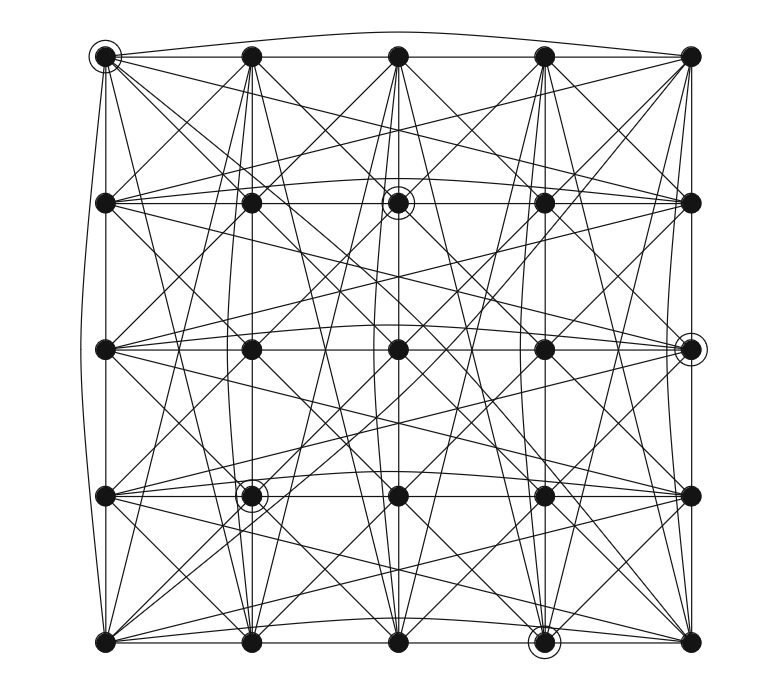
\includegraphics[width=\marginparwidth-20pt]{images/C5xC6.png}\ \ \ \center The graph $C_5 \times C_6$.}

\noindent and Shannon's problem was to compute $\Theta(G)$, and in particular $\Theta(C_5)$.


Let us look at $C_5$. So far we know $\alpha(C_5) = 2 \leq \Theta(C_5)$. Looking at 
the $5$-cycle as depicted earlier, or at the product $C_5 x C_5$ as drawn on the 
left, we see that the set $\{(1, 1), (2,3), (3,5), (4,2), (5,4)\}$ is independent 
in $C_5^2$. Thus we have $\alpha(C_5^2) \geq 5$. Since an independent set can contain 
only two vertices from any two consecutive rows we see that $\alpha(C_5^2) = 5$.
Hence, by using strings of length $2$ we have increased the lower bound for the capacity to $\Theta(C_5) \geq \sqrt{5}$.


\noindent So far we have no upper bounds for the capacity. To obtain such bounds 
we again follow Shannon's original ideas. First we need the dual definition 
of an independent set. We recall that a subset $C \subseteq V$ is a \textit{clique} if any
two vertices of $C$ are joined by an edge. Thus the vertices form trivial

\setsecondpagemargins

\noindent cliques of size $1$, the edges are the cliques of size $2$, the triangles are cliques 
of size $3$, and so on. Let $C$ be the set of cliques in $G$. Consider an arbitrary 
probability distribution $x = (x, : v \in V)$ on the set of vertices, that 
is, $x_v \geq 0$ and $\sum_{v \in V} x_v = 1$. To every distribution $x$ we associate 
the ``maximal value of a clique"

\begin{equation*}
\lambda(x) = \max_{C \in \mathcal{C}} \sum_{v\in C} x_v.
\end{equation*}

\noindent and finally we set

\begin{equation*}
\lambda(G) = \min_x\lambda(x) = \min_x\max_{C \in \mathcal{C}} \sum_{v\in C} x_v.
\end{equation*}

\noindent To be precise we should use inf instead of min, but the minimum exists
because $\lambda(x)$ is continuous on the compact set of all distributions.
Consider now an independent set $U \subseteq V$ of maximal size $\alpha(G) = \alpha $.
Associated to $U$ we define the distribution $x_U  = (x_v : v \in V)$ by setting 
$x_v = \frac{1}{\alpha}$ if $v \in U$ and $x_v = 0$ otherwise. Since any clique contains at most 
one vertex from $U$,  we infer $\lambda(x_U) = \frac{1}{\alpha} $, 
and thus by the definition of $\lambda(G)$

\begin{equation*}
\lambda(G) \leq \frac{1}{\alpha(G)} \quad \text{or} \quad \alpha(G) \leq \lambda(G)^{-1}.
\end{equation*}

What Shannon observed is that $\lambda(G)^{-1}$ is, in fact, an upper bound for all 
$\sqrt[n]{\alpha(G^n)}$, and hence also for $\Theta(G)$. In order to prove this it suffices to 
show that for graphs $G$, $H$

\begin{equation}
\lambda(G \times H) = \lambda(G)\lambda(H) \label{one}
\end{equation}

holds, since this will imply $\lambda(G^n) = \lambda(G)^n$ and hence

\begin{equation*}
  \begin{align*}
  \alpha(G^n) \leq \lambda(G^n)^{-1} = \lambda(G)^{-n} \\
  \sqrt[n]{\alpha(G^n)} \leq \lambda(G)^{-1}.
  \end{align*}
\end{equation*}

% FIX BIBLIOGRAPHY
To prove (\ref{one}) we make use of the duality theorem of linear programming 
(see [I]) and get

\begin{equation}
  \lambda(G) = \min_x\max_{C \in \mathcal{C}} \sum_{v\in C} x_v = \max_y\min_{v \in V}\sum_{C \ni v}y_C, \label{two}
\end{equation}

\noindent where the right-hand side runs through all probability distributions $y = (y_C : C \in \mathcal{C})$
on $\mathcal{C}$.\\
Consider $G \times H$, and let $x$ and $x'$ be distributions which achieve the 
minima, $\lambda(x) = \lambda(G)$, $\lambda(x') = \lambda(H)$. In the vertex set of $G \times H$ we 
assign the value $z_{(u,v)} = x_ux'_v$ to the vertex $(u, v)$. Since $\sum_{(u,v)}z_{(u,v)} = \sum_u x_u \sum_v x'_v, = 1$, 
we obtain a distribution. Next we observe that the maximal cliques in 
$G \times H$ are of the form $C \times D = \{(u, v) : u \in C, v \in D \} $
where $C$ and $D$ are cliques in $G$ and $H$, respectively. Hence we obtain 

\begin{equation*}
  \begin{align}
  \lambda(G \times H) \leq \lambda(z) = \max_{C \times D} \sum_{(u,v) \in C \times D} z_(u,v)\\
  - \max_{C \times D} \sum_{u\in C} x_u \sum_{v \in D} x'_v = \lambda(G)\lambda(H)
  \end{align}
\end{equation*}

\end{document}

